%!TEX root = ./template-skripsi.tex
%-------------------------------------------------------------------------------
%                            BAB II
%               KAJIAN TEORI
%-------------------------------------------------------------------------------

\chapter{KAJIAN TEORI}                

Kumpulan resep masakan pada umumnya memuat berbagai macam makanan yang siap untuk dimasak. Makanan merupakan elemen penting yang membentuk suatu resep karena makanan adalah produk hasil akhir yang ingin dicapai melalui panduan yang terdapat dalam resep masakan. Resep masakan kemudian dijadikan konten utama dalam pengembangan yang dilakukan oleh penulis dengan menggunakan Android sebagai wadah bagi aplikasi atau perangkat lunak tersebut. Pengembangan resep masakan ini dilakukan berdasarkan tahapan \emph{System Development Life Cycle} (SDLC) yang berlaku secara umum dalam dunia \emph{software developing}.


\section{Pengembangan Aplikasi Perangkat Lunak}
	Pengembangan perangkat lunak pada umumnya sama dengan membangun sebuah gedung. Proses pertama dimulai dengan sebuah ide atau gagasan, lalu dilanjutkan dengan merubah ide atau gagasan tersebut menjadi sebuah desain sehingga dapat memberi gambaran lebih jelas tentang ide tersebut. Proses selanjutnya bersifat opsional, yakni melakuan revisi atau perubahan terhadap desain apabila dirasa tidak sesuai dengan yang diinginkan. Setelah itu, dilanjutkan dengan melakukan pembuatan cetak biru terhadap desain tersebut sehingga memperoleh gambaran yang lebih mendetail lagi dari masing-masing bagian gedung tersebut. Proses yang terakhir adalah membangun gedung tersebut berdasarkan cetak biru yang ada \cite{francis}. 
	
	Dalam proses pengembangan aplikasi perangkat lunak, terdapat istilah SDLC atau \emph{System Development Life Cycle}. SDLC adalah sebuah metode atau proses untuk memberikan pengertian bagaimana sebuah sistem informasi dapat mendukung kebutuhan bisnis dengan melakukan desain sebuah sistem, membangun sistem tersebut, dan mengimplementasikannya ke pengguna \cite{denis}.
	
	SDLC memiliki 4 tahapan utama yakni perencanaan, analisa, desain, dan implementasi. Dalam sebuah proyek pengembangan aplikasi perangkat lunak pastilah memiliki keempat tahapan tersebut, namun cara untuk melaksanakan tahapan-tahapan tersebut dapat berbeda-beda antara satu proyek dengan proyek lainnya. Setiap tahapan tersebut memiliki langkah-langkah tersendiri dalam menjalankan tahapan-tahapan tersebut sesuai dengan tujuan akhir dari masing-masing tahapan tersebut.
	
	\begin{figure}[H]
		\centering
		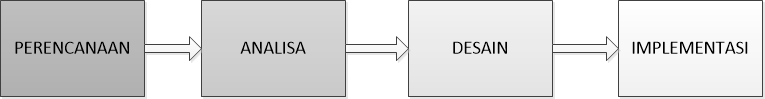
\includegraphics[width=1\textwidth]{gambar/sdlc_overview}
		\caption{Empat Tahapan Utama SDLC}
		\label{sdlc_overview}
	\end{figure}
		
	Jenis-jenis pelaksanaan dari tahapan-tahapan SDLC terdiri dari \cite{pressman}:
	\begin{enumerate}
		\item \emph{Linear Process Flow}, yang mengeksekusi 4 tahapan tersebut secara berurutan
		\item \emph{Iterative Process Flow}, yang mengeksekusi secara berulang satu atau beberapa tahapan sebelum melanjutkan ke tahapan selanjutnya
		\item \emph{Evolutionary Process Flow}, mengeksekusi tahapan tersebut secara melingkar
		\item \emph{Parallel Process Flow}, mengeksekusi satuu atau beberapa tahapan secara bersamaan dengan tahapan lain. 
	\end{enumerate}

	Dalam metode SDLC terdapat beberapa model pengembangan yang dapat dijadikan acuan dasar kerangka kerja dalam proses pengembangan sebuah aplikasi perangkat lunak, yakni \emph{Waterfall Model}, \emph{Iterative Model}, \emph{Spiral Model}, \emph{V-Model}, \emph{Big Bang Model}, \emph{Agile Model}, \emph{Rapid Application Development (RAD) Model}, dan \emph{Prototyping Model}. Dalam pengembangan aplikasi resep masakan ini, penulis memilih menggunakan \emph{Spiral Model}.
	
	Model spiral memadukan sistematika dari pembangunan antara model iteratif (\emph{Iterative Model}) dengan aspek pengendalian dari model \emph{waterfall} (\emph{Waterfall Model}). Model spiral termasuk dalam jenis \emph{Evolutionary Process Flow}, yang mengeksekusi tahapan pengerjaan secara melingkar \cite{tutorialspoint}. Tahapan-tahapan yang akan dilakukan dalam penelitian ini mengikuti model pengembangan spiral, yaitu: \emph{Identification} (identifikasi kebutuhan), \emph{Design} (Desain Sistem), \emph{Construct and Build} (Pembuatan Sistem), dan \emph{Evaluation} (\emph{delivery feedback and release})
    \begin{figure}[H]
		\centering
		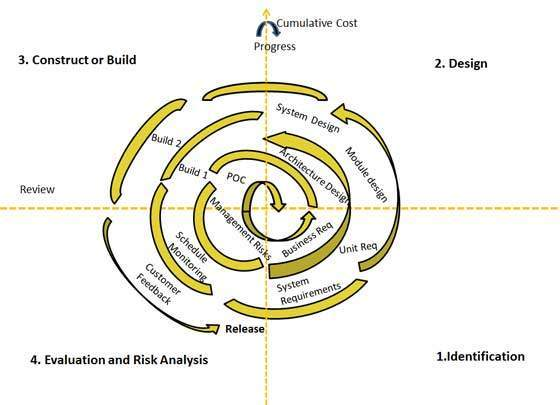
\includegraphics[width=0.6\textwidth]{gambar/sdlc_spiral_model}
		\caption{Model Spiral}
		\label{sdlc_spiral_model}
	\end{figure}

	Penulis memilih menggunakan model spiral sebagai model dari SDLC dalam proses pengembanga aplikasi kumpulan resep masakan terkoneksi \textit{food channel} YouTube dengan alasan apabila dalam proses pengembangan terdapat kesalahan, baik dalam proses identifikasi, desain, atau pembuata sistem, maka penulis dapat kembali ke tahap dimana ditemukan kesalahan untuk kemudian memperbaiki kesalahan tersebut sehingga proses pegembangan dapat dilaksanakan secara semestinya dan penulis juga tidak melanggar ketentuan yang telah ditetapkan oleh metode pengembangan SDLC karena fleksibilitas dari model spiral itu sendiri.

\section{\emph{Unified Modeling Language} (UML)}
	\emph{Unified Modeling Language} atau UML adalah sebuah Bahasa pemodelan terstandarisasi dan digunakan untuk berbagai kebutuhan dalam memodelkan pembuatan \emph{software}yang berorientasi pada obyek (\emph{object-oriented}). Standar tersebut dbuat dan dikelola oleh Object Management Group (OMG) pada tahun 1997 dan telah menjadi standar di bidang industri pembuatan \emph{software}. UML meliputi sebuah set dari teknik notasi grafis untuk membuat model dari sebuah sistem perangkat lunak berorientasi obyek secara visual. UML juga merupakan peralatan untuk menspesifikasikan dan memvisualisasikan sebuah sistem pada perangkat lunak. Hal tersebut mencakup tipe diagram yang telah terstandarisasi untuk mendeskripsikan serta memetakan sebuah aplikasi komputer atau desain serta struktur dari sebuah sistem basis data. UML memiliki fungsi untuk mengelola sistem yang besar dan kompleks. Memiliki struktur aplikasi yang jelas dapat membantu \emph{developer} dalam mengenalkan proyek kepada orang-orang baru maupun awam \cite{lee}.
	
	Jenis UML yang digunakan oleh peneliti pada pengembangan aplikasi ini adalah \emph{Use Case Diagram}, \emph{Class Diagram}, dan \emph{Activity Diagram}.
	
	\subsection{\emph{Use Case Diagram}}
		Fungsionalitas dari sebuah sistem basis data maupun sebuah perangkat lunak komputer dapat diilustrasikan dengan diagram \emph{use case}. Tugas utama dari sebuah \emph{use case} adalah memvisualisasikan kebutuhan fungsionalitas dari sebuah sistem, termasuk hubungan antara aktor (orang yang akan berinteraksi dengan sistem) dengan proses-proses yang esensial dalam sebuah sistem untuk mencapai suatu tujuan. Hal tersebut dapat dikategorikan sebagai kumpulan langkah-langkah yang mendefinisikan interaksi antara aktor dan sistem \cite{bell}.  
		
		\vspace{1cm}
		
		\textit{Use Case Diagram} terdiri dari beberapa komponen, yakni:
		\begin{enumerate}
			\item Aktor\\ 
			Menggambarkan seorang aktor atau pengguna sistem yang akan berinteraksi dengan sistem
			\begin{figure}[H]
				\centering
				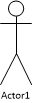
\includegraphics[width=0.05\textwidth]{gambar/use-case/aktor}
				\caption{Aktor dalam \textit{Use Case}}
			\end{figure}
			\item Oval\\ 
			Bentuk Oval menggambarkan sistem yang dapat berinteraksi dengan aktor. Bentuk Oval tersebut biasanya disertai dengan nama aktivitas sistem di dalamnya yang terletak ditengah-tengah bentuk oval tersebut
			\begin{figure}[H]
				\centering
				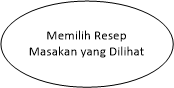
\includegraphics[width=0.4\textwidth]{gambar/use-case/balon}
				\caption{Sistem dengan Bentuk Oval}
			\end{figure}
		
			\item Garis Penghubung Aktor dan Sistem\\ 
			Untuk menggambarkan interaksi antara Aktor dan Sistem, diperlukan sebuah garis yang menghubungkan antara aktor dan sistem. Sebuah garis digunakan untuk menghubungkan keduanya
			\begin{figure}[H]
				\centering
				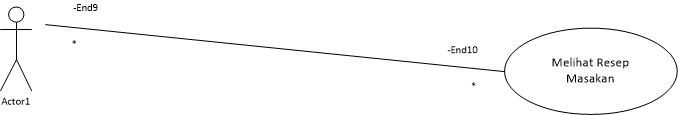
\includegraphics[width=0.8\textwidth]{gambar/use-case/penghubung_aktor_sistem}
				\caption{Garis Penghubungan antara Aktor dan Sistem}
				\label{garis_aktor_sistem}
			\end{figure}
			Gambar \ref{garis_aktor_sistem} memperlihatkan garis yang menyambungkan aktor dengan interaksi sistem menyatakan bahwa Aktor dapat Melihat Resep Masakan
			
			\item Garis Penghubung Antar Sistem\\ 
			Sistem yang terdapat pada \textit{use case} dapat berinteraksi satu sama lain. Terdapat dua jenis hubungan antar sistem, yakni \textit{include} dan \textit{extend}. Sesuai dengan namanya, \textit{include} menyatakan bahwa sebuah interaksi sistem yang terhubung adalah bagian dari interaksi sistem lainnya
			\begin{figure}[H]
				\centering
				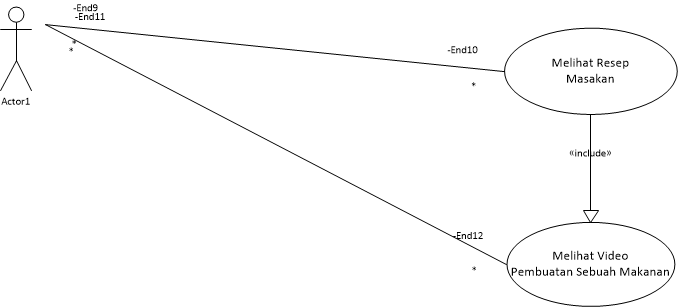
\includegraphics[width=1\textwidth]{gambar/use-case/include}
				\caption{Contoh Hubungan \textit{Include}}
				\label{hub_include}
			\end{figure}
			Gambar \ref{hub_include} menjelaskan bahwa Melihat Video Pembuatan Sebuah Makanan merupakan bagian dari Melihat  Resep Masakan. Sedangkan penghubung \textit{extend} menyatakan bahwa interaksi sebuah sistem merupakan perluasan dari interaksi sistem lainnya
			\begin{figure}[H]
				\centering
				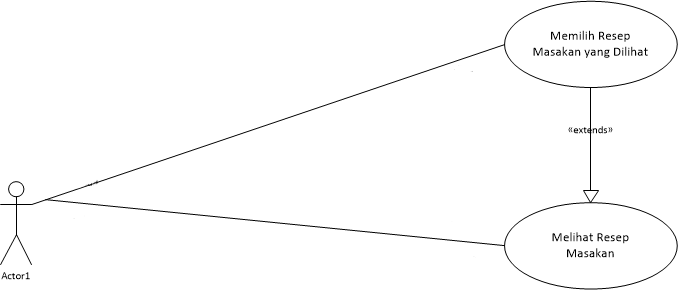
\includegraphics[width=1\textwidth]{gambar/use-case/extends}
				\caption{Contoh Hubungan \textit{Extend}}
				\label{hub_extend}
			\end{figure}
			Gambar \ref{hub_extend} menjelaskan bahwa Melihat Resep Masakan merupakan perluasan dari Memilih Resep Masakan yang Dilihat. Sebagai contoh, seorang Aktor dapat berinteraksi dengan sebuah sistem berbentuk aplikasi resep masakan. Interaksi yang dimungkinkan oleh sistem adalah Memilih Resep Masakan, Melihat Resep Masakan, dan Melihat Video Pembuatan Sebuah Resep Masakan. \textit{Use Case} dari interaksi tersebut terdapat pada Gambar \ref{use-case-example}. Gambar tersebut menjelaskan bahwa aktor dapat memilih resep masakan dan kemudian juga melihat resep masakan yang telah dipilih. Melihat resep masakan yang dipilih merupakan ekstensi dari interaksi antara akor denga sistem yaki memilih resep masakan yang dilihat. Kemudian pengguna juga dapat melihat video pembuatan sebuah makanan ketika melihat resep masakan. Hal tersebut dimungkinkan karena interaksi melihat resep masakan memiliki hubungan \textit{include} dengan innteraksi melihat video pembuatan sebuah makanan.
			\begin{figure}[H]
				\centering
				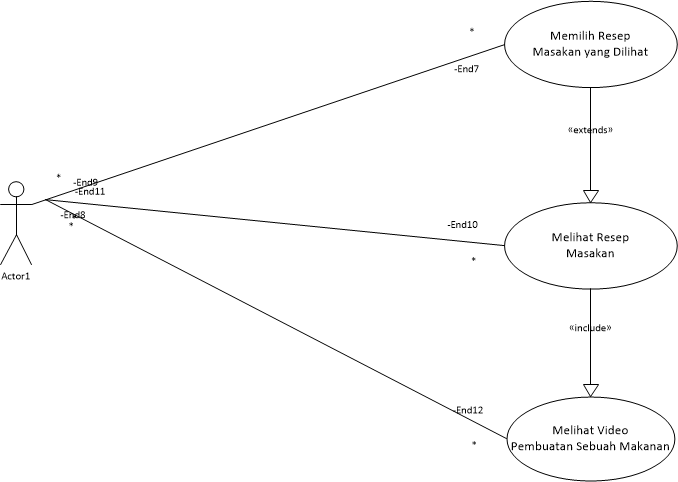
\includegraphics[width=1\textwidth]{gambar/use-case/contoh-use-case}
				\caption{Contoh \textit{Use Case} dalam Penggunaan Aplikasi Resep Masakan}
				\label{use-case-example}
			\end{figure}
			Jadi, dapat disimpulkan bahwa Use Case Diagram adalah sebuah diagram yang menggambarkan interaksi antara Aktor (pengguna) dengan sistem yang digunakan oleh Aktor.
			  

		\end{enumerate}
		
		
	\subsection{\emph{Class Diagram}}
		Struktur statis dari sebuah aplikasi komputer atau pangkalan basis data dapat digambarkan melalui sebuah \emph{class diagram}. \emph{Class diagram} juga menunjukkan perbedaan entitas (pengguna, alat, maupun data) yang berelasi satu sama lain. Diagram tersebut biasa digunakan untuk menampilkan class-class secara logikal, dan untuk mengimplementasikan class yang telah dibuat. \emph{Class diagram} merupakan unsur terpenting dalam pemodelan aplikasi berbasis obyek (\emph{object-oriented}) dan merupakan sebuah tipe struktur diagram statis yang mendeskripsikan struktur dari sebuah sistem dengan menampilkan \emph{class} dari sistem, atribut, operasi (method), dan relasi antar \emph{class} \cite{lee}.  
		
	\subsection{\emph{Activity Diagram}}
		Kontrol alur serta prosedur antara dua atau lebih obyek \emph{class} dalam memproses sebuah aktivitas dapat ditunjukkan melalui sebuah \emph{activity diagram}. Diagram tersebut dapat digunakan untuk memodelkan proses bisnis tingkat atas dalam sebuah level unit bisnis, atau untuk memodelkan aksi-aksi dalam class internal yang bersifat \emph{low level} (Bell, 2003). \emph{Activity Diagram} adalah representasi grafis dari sebuah alur pengerjaan yang berupa tahap-tahap dari berbagai aktivitas serta aksi dengan dukungan pilihan, iterasi, dan persetujuan. Pada UML, \emph{activity diagram} dapat digunakan untuk mendeskripsikan bisnis serta langkah-langkah operasional serta alur pengerjaan dari berbagai komponen yang berada dalam sebuah sistem. Sebuah \emph{activity diagram} menjelaskan keseluruhan alur dari sebuah sistem \cite{lee}. Contoh dibawah ini menjelaskan aktivitas pemrosesan pesanan dalam sebuah sistem Point of Sales (POS).  
		\begin{figure}[H]
			\centering
			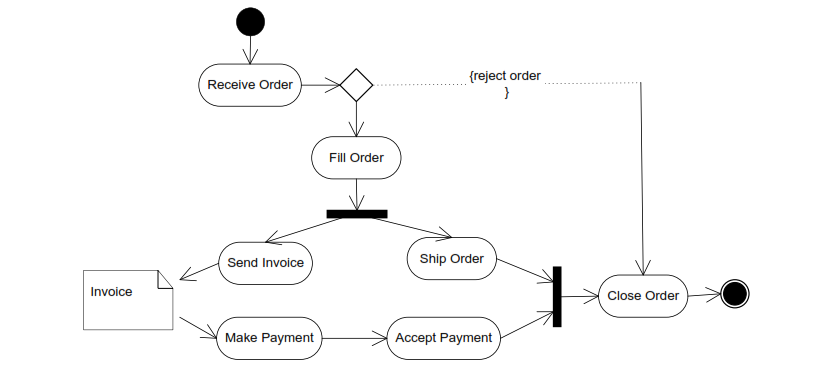
\includegraphics[width=1\textwidth]{gambar/sample-activity-diagram}
			\caption{Contoh \textit{Activity Diagram} dalam sistem Point Of Sales (POS)}
		\end{figure}
\section{\emph{Structured Query Language} (SQL)}
	SQL merupakan singkatan dari \emph{Structure Query Language}, didefinisikan sebagai suatu sintaks perintah-perintah tertentu atau bahasa program yang digunakan untuk mengelola suatu \emph{database} \cite{anisya}. SQL adalah sebuah konsep pengoperasian \emph{database}, terutama untuk pemilihan atau seleksi dan pemasukan data, yang memungkinkan pengoperasian data dikerjakan dengan mudah secara otomatis. Keandalan suatu sistem \emph{database} (DBMS) dapat diketahui dari cara kerja \emph{optimizer}-nya dalam melakukan proses perintah-perintah SQL, yang dibuat oleh user maupun program-program aplikasinya. 
	Query dikirimkan ke database dalam bentuk SQL Query Beberapa perintah yang umum digunakan adalah sebagai berikut:
	
	\begin{enumerate}
		\item 
		CREATE : Untuk membuat tabel baru
		\begin{figure}[H]
			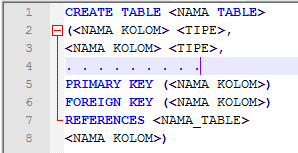
\includegraphics[width=0.4\textwidth]{gambar/sql/create}
		\end{figure}
		\item
		SELECT : Untuk mengambil \textit{record} dari database yang memenuhi kriteria tertentu
		\begin{figure}[H]
			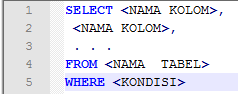
\includegraphics[width=0.5\textwidth]{gambar/sql/select}
		\end{figure} 
		\item
		INSERT : Untuk menambah \textit{record} ke dalam suatu tabel
		\begin{figure}[H]
			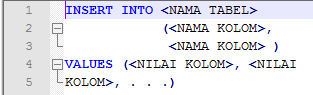
\includegraphics[width=0.5\textwidth]{gambar/sql/insert}
		\end{figure}
		\item
		UPDATE : Untuk merubah isi \textit{record} tertentu pada suatu tabel
		\begin{figure}[H]
			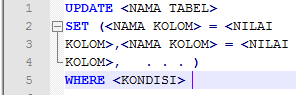
\includegraphics[width=0.5\textwidth]{gambar/sql/update}
		\end{figure}
		\item
		DELETE : Untuk menghapus \textit{record} pada suatu tabel
		\begin{figure}[H]
			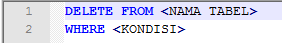
\includegraphics[width=0.5\textwidth]{gambar/sql/delete}
		\end{figure} 
		\item
		DROP : Untuk menghapus sebuah tabel
		\begin{figure}[H]
			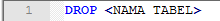
\includegraphics[width=0.5\textwidth]{gambar/sql/drop}
		\end{figure}
		\item
		JOIN : Untuk menggabungkan dua atau lebih tabel
		\begin{figure}[H]
			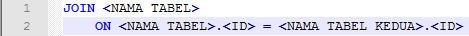
\includegraphics[width=0.8\textwidth]{gambar/sql/join}
		\end{figure}
	\end{enumerate}
		
\section{\emph{Entity Relationship Diagram} (ERD)}
	\emph{Entity Relationship Diagram} (ERD) adalah sekumpulan cara atau peralatan untuk mendeskripsikan data-data atau objek-objek yang dibuat berdasarkan dan berasal dari dunia nyata yang disebut entitas (\emph{entity}) serta relasi (\emph{relationship}) antar entitas-entitas tersebut dengan menggunakan beberapa notasi \cite{edi}. Komponen-komponen pembentuk ERD dapat dilihat pada Tabel \ref{tabel_komponen_erd}. 
	\begin{table}[H]
		\centering
		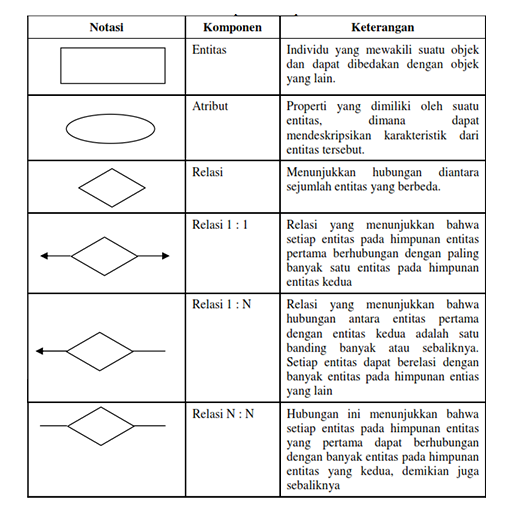
\includegraphics[width=0.8\textwidth]{gambar/erd/erd}
		\caption{Komponen-komponen Pembentuk ERD}
		\label{tabel_komponen_erd}
	\end{table}
	Sesuai dengan namanya, sebuah ERD memodelkan data sebagai entitas serta relasi (\emph{relationship}). Entitas adalah data yang ingin disimpan. Chen (1976) dalam presentasinya mendeskripsikan entitas sebagai  "sesuatu yang dapat diidentifikasi secara jelas." Jadi, entitas dapat berupa seseorang, sebuah tempat, obyek, kejadian, atau konsep yang ingin disimpan sebagai data. 
	
	Relasi (\emph{relationship}) adalah koneksi antara entitas-entitas yang ada. Relasi sendiri memiliki kardinalitas, yaitu ukuran kasar dari jumlah entitas (satu atau lebih) yang akan terkait dengan entitas lain (atau entitas). Berdasarkan kardinalitasnya, terdapat tiga jenis relasi yang dapat ditemukan dalam entitas-entitas yang ada yaitu relasi \emph{one-to-one} (1:1), \emph{one-to-many} (1:M), dan \emph{many-to-many} (M:N). Dalam relasi \emph{one-to-one}, sebuah entitas dapat berasosiasi dengan satu entitas lainnya dan sebaliknya. Contohnya, seorang siswa hanya memiliki satu sepeda. Dengan analogi antara siswa dengan sepeda tersebut, relasi \emph{one-to-many} menggambarkan bahwa seorang siswa dapat memiliki banyak sepeda. Sedangkan relasi \emph{many-to-many} pada analogi siswa dengan sepeda adalah banyak siswa yang dapat memiliki banyak sepeda dan sebaliknya \cite{bagui}. 
	
	Atribut adalah kategori dari sebuah data yang mendeskripsikan sebuah entitas atau relasi. Contoh dari atribut adalah sebuah entitas bernama MOBIL memiliki atribut tipe, warna, id\_kendaraan, dan lain sebagainya. Basis data sering digunakan untuk menyimpan data yang akan digunakan pada tahapan-tahapan selanjutnya. Sebuah atribut yang dapat digunakan untuk mencari suatu entitas tertentu disebut kunci atau \emph{key}. Atribut yang bersifat kunci (\emph{key}) dapat muncul secara natural apabila sebuah basis data dimodelkan dengan menggunakan ERD. Jika sebuah atribut dapat diperhitungkan menjadi sebuah ciri khas dari suatu entitas karena keunikannya, maka atribut tersebut disebut dengan \emph{candidate key} atau kandidat kunci. \emph{Candidate key} akan berubah menjadi \emph{primary key} apabila telah dipilih sebagai atribut khas suatu entitas yang bersifat paling unik daripada atribut lain yang terdapat pada suatu entitas.
	
	\subsection*{Studi Kasus Minimarket}
	Sebuah minimarket yang menjual berbagai jenis barang kebutuhan sehari-hari
	memiliki sebuah sistem informasi untuk mengelola penjualan secara langsung
	(point of sales), pengadaan barang, dan \textit{stock control}. Proses bisnis dalam penjualan barangnya dimulai pada saat \textit{customer} memilih barang yang akan dibeli. Setelah \textit{customer} memutuskan untuk membeli barang tersebut, maka kasir akan meminta informasi tentang identitas \textit{customer} untuk dicatat jika \textit{customer} yang bersangkutan terdaftar sebagai member. Namun jika \textit{customer} tersebut bukanlah member minimarket, maka data-data \textit{customer} akan diabaikan. Kemudian kasir akan membuatkan nota penjualan barang. Setelah barang diterima oleh \textit{customer}, \textit{customer} akan melakukan pembayaran. Proses berakhir ketika kasir memberikan bukti pembayaran kepada \textit{customer}. Sistem informasi yang tersedia tidak melayani proses pengembalian barang dan pemesanan barang. 
	Proses bisnis untuk pembelian barang dari supplier dimulai ketika pihak minimarket menghubungi supplier dan memesan barang. \textit{Supplier} kemudian akan membuatkan nota pembelian. Barang yang sudah dipesan lalu akan diantarkan ke minimarket.  Jika  barang  sudah  diterima,  maka  proses  yang  terjadi  adalah pembayaran dari pihak minimarket ke pihak \textit{supplier}. Setelah semua proses pembayaran  selesai,  \textit{supplier}  akan  memberikan  bukti  pembayaran  dan  proses selesai. Seperti halnya pada proses penjualan, proses pembelian tidak menangani pengembalian barang kepada \textit{supplier}. 
	Untuk proses \textit{stock control}, dilakukan proses pencatatan terhadap barang yang di- supply, barang yang dibeli oleh \textit{customer} dan sisa barang yang ada di gudang per harinya. Hal ini dimaksudkan agar setiap keluar masuknya barang yang ada dapat terawasi dan menjaga barang selalu tersedia di gudang. 
	Maka ERD yang dapat dibuat dari kasus diatas adalah sebagai berikut:
	\begin{figure}[H]
		\centering
		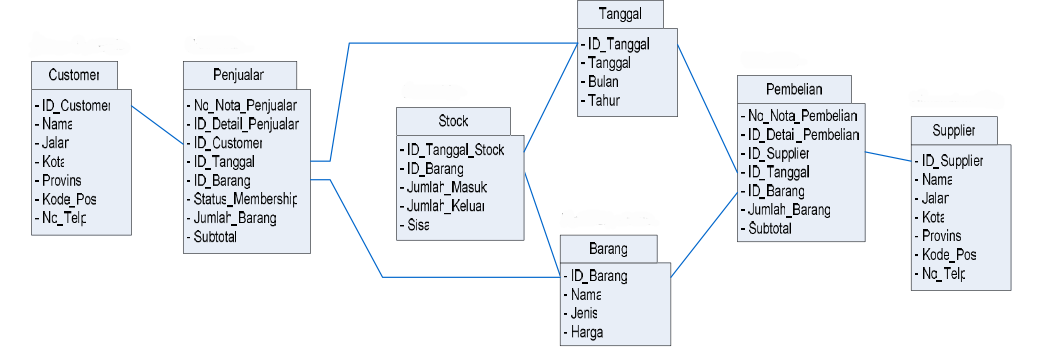
\includegraphics[width=1.1\textwidth]{gambar/erd/sample-erd}
		\caption{ERD Studi Kasus Minimarket}
	\end{figure}
	
	
	
\section{Pengertian Android}
	Android adalah sebuah sistem operasi untuk perangkat \emph{mobile} berbasis linux yang mencakup sistem operasi, \emph{middleware} dan aplikasi. Android menyediakan \emph{platform} terbuka bagi para pengembang untuk menciptakan aplikasi mereka \cite{murtiwiyati}. Dikutip dari situs resmi Open Handset Alliance, yang merupakan pengembang sistem operasi Android pertama di dunia, Android dikembangkan untuk memungkinkan para pengembang aplikasi membuat suatu aplikasi \emph{mobile} yang dapat memanfaatkan seluruh kelebihan yang ditawarkan dari suatu perangkat \emph{mobile}. Android dibuat secara terbuka dan semua orang dapat mengembangkan dan menggunakan semua fungsionalitasnya. Contohnya, sebuah aplikasi yang dapat digunakan untuk melakukan berbagai macam fungsionalitas sebuah ponsel seperti membuat panggilan, mengirimkan pesan singkat, atau mengambil gambar dengan kamera, memungkinkan para pengembang aplikasi untuk membuat banyak sekali fitur lainnya yang dapat digunakan oleh para penggunanya. Android dibuat dengan menggunakan Kernel Linux yang bersifat terbuka (\emph{open source}). Selain itu, Android juga merupakan hasil dari modifikasi mesin virtual (\emph{virtual machine}) yang didesain untuk mengoptimalkan memori serta perangkat keras (\emph{hardware}) pada sebuah ponsel. Android sendiri adalah open source yang berarti dapat terus dikembangkan menjadi sebuah teknologi baru sesuai dengan kebutuhan manusia pada saat ini. \emph{Platform} ini akan terus berkembang seiring dengan pergerakan para pengembang aplikasi yang bekerja bersama-sama untuk membangun aplikasi \emph{mobile} yang inovatif. 
	
	Gambar \ref{android-sbg-platform} menunjukkan hirarki aplikasi yang dibuat oleh peneliti terhadap \textit{platform} Android.   
	
	\begin{figure}[H]
		\centering
		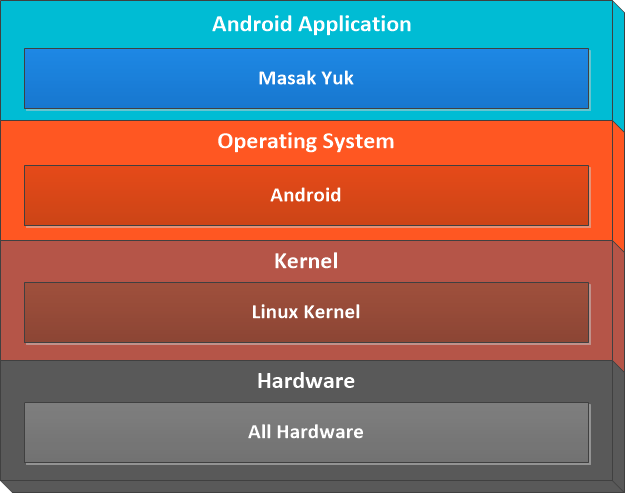
\includegraphics[width=1\textwidth]{gambar/stack-diagram-bab-2}
		\caption{\textit{Stack Diagram} Hirarki Aplikasi Android dengan Komponen Lainnya}
		\label{android-sbg-platform}
	\end{figure}
	

	Selain kemampuannya untuk mendukung dan memfasilitasi berbagai fungsi familiar seperti membuat panggilan, berkirim pesan elektronik, dan mencari sebuah restoran, perangkat Android dapat menjadi sebuah perangkat dengan fungsi tanpa batas dan dapat dikembangkan kapan saja bergantung pada pemikiran para pengembangnya \cite{rogers}. Saat ini, Android tidak hanya terdapat pada sebuah ponsel tetapi juga tertanam dalam sebuah tablet, televisi, kacamata pintar, kulkas, mobil dan lain sebagainya. Jadi dapat disimpulkan bahwa Android merupakan sistem operasi untuk sebuah perangkat cerdas yang dapat memiliki banyak fitur dan fungsi sesuai dengan keinginan para pengembangnya untuk menjawab masalah-masalah yang terdapat dalam kehidupan manusia. 

\section{Android Studio}
	Android Studio merupakan sebuah \emph{Integrated Developing Environment} (IDE) untuk \emph{platform} Android. Android Studio ini diumumkan pada tanggal 16 Mei 2013 pada konferensi Google I/O oleh \emph{Product Manager} Google, Ellie Powers. Android Studio bersifat \emph{free} dibawah Apache \emph{License} 2.0. Versi awal Android Studio yaitu 0.1 dirilis pada bulan Mei 2013. Kemudian dibuat versi \emph{beta} 0.8 yang dirilis pada bulan Juni 2014. Versi yang paling stabil dirilis pada bulan Desember 2014, dimulai dari versi 1.0. Berbasiskan JetBrainns' IntelliJ IDEA, Studio di desain khusus untuk Android \emph{Development}. Android Studio sudah bisa diunduh untuk Windows, Mac OS X, dan Linux

	Berikut ini adalah beberapa keunggulan Android Studio:
	\begin{enumerate}
		\item Android \emph{Memory} (HPROF) \emph{Viewer}\\
		Android Studio kini mengizinkan penggunanya untuk menangkap dan menganalisa \emph{snapshot} memori dalam format Android HPROF.
		\item \emph{Allocation Tracker}\\
		Untuk mempermudah dalam menganalisa penggunaan alokasi memori aplikasi yang dibuat oleh penggunanya, \emph{Allocation Tracker} kini menambahkan fitur visual. Dengan adanya fitur ini, alokasi memori yang digunakan oleh aplikasi yang dibuat oleh penggunanya dapat terlihat dalam diagram berbentuk lingkaran.
		\item APK \emph{Test}\\
		Kini plugin baru ('com.android.test') telah ditambahkan untuk mempermudah penggunanya dalam mencoba atau melakukan \emph{testing} aplikasi Android yang sedang dikembangkan. Untuk menggunakan fitur ini, penggunanya harus memiliki Gradle Plugin versi 1.3.
		\item \emph{Application Permission Annotation}\\
		Android Studio (sejak versi 1.3) mendukung \emph{inline code annotation} yang akan membantu penggunanya mengatur \emph{app permission} yang dirilis pada Android M (Android 6.0/Marshmallow).
		\item SDK \emph{Auto Update} dan SDK \emph{Manager}
		Android Studio mengatur pembaharuan SDK dan plugin-plugin lainnya secara otomatis.
	\end{enumerate}

\section{\emph{Application Programming Interface} (API)}
	\emph{Application Programming Interfaces} atau biasa disingkat API, yang didalamnya termasuk kumpulan \emph{library}, \emph{framework}, peralatan penunjang (\emph{toolkits}), dan peralatan pengembangan \emph{software} lainnya, digunakan secara virtual dalam semua bahasa pemrograman \cite{myers}. Jika sebuah perangkat lunak mengandung API \emph{internal} (yang berasal dari dalam perangkat lunak tersebut) serta API publik (seperti Java Platform SDK, Windows .NET Framework, jQuery untuk JavaScript, dan Web services seperti Google Map), maka setiap baris dari kode yang ditulis oleh \emph{programmer} memanggil dan menggunakan API. API menyediakan sebuah mekanisme dalam penggunaan kembali sebuah kode yang telah dibuat sebelumnya sehingga \emph{programmer} dapat memanfaatkannya kembali untuk keperluan yang berbeda. Hal ini sangat efektif apabila dibandingkan dengan membuat setiap program dan kode dari awal. Lebih lanjut lagi, penggunaan API sangat dibutuhkan karena akses yang bersifat \emph{low-level} menuju kepada sebuah sumber dari suatu sistem (seperti grafik atau gambar, \emph{networking}, dan \emph{file} sistem) yang tersedia hanya melalui API yang terproteksi.
	
	\begin{figure}[H]
		\centering
		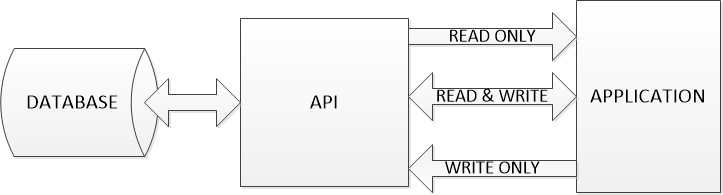
\includegraphics[width=1\textwidth]{gambar/api/api_chart}
		\caption{Cara Kerja API}
	\end{figure}

	API menjembatani sebuah basis data dengan aplikasi yang mengakses basis data tersebut. Terdapat tiga jenis metode yang dihasilkan oleh API, yaitu metode \textit{read only} (hanya membaca), \textit{write only} (menulis atau mengubah saja), dan \textit{read and write} (membaca dan menulis atau mengubah data). Ketiga jenis metode tersebut dibuat sesuai dengan kebutuhan aplikasi yang akan dijembatani oleh API.   
	 
	
\section{Integrasi YouTube dengan Aplikasi Android}
	YouTube dapat diintegrasikan ke dalam sebuah aplikasi Android dengan mengimplementasikan API (\emph{Application Programming Interface}) yang disediakan oleh YouTube dan Google secara gratis (\emph{open source}) yang berarti semua orang dapat menggunakannya tanpa terkecuali. API tersebut dinamakan YouTube Android Player API.
	
	Dilansir dari situs Google Developer, API tersebut memungkinkan penggunanya untuk memasukkan fungsi pemutaran video ke dalam aplikasi Android. API tersebut mendefinisikan metode untuk menampilkan dan memainkan video-video YouTube (dan juga \emph{playlist}) dan untuk memodifikasi serta mengatur pemutaran video dalam aplikasi Android.
	
	\begin{figure}[H]
		\centering
		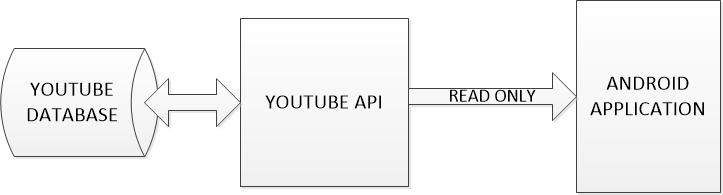
\includegraphics[width=1\textwidth]{gambar/api/youtube_api_chart}
		\caption{Cara Kerja YouTube API}
	\end{figure}

	YouTube Android Player API termasuk dalam jenis API yang menyediakan \textit{read only method}, yaitu API yang menyediakan metode untuk membaca data yang terdapat dalam sebuah basis data, dimana basis data yang digunakan pada aplikasi ini adalah basis data YouTube. Video dialirkan kedalam aplikasi Android menggunakan berbagai macam metode yang terdapat dalam API YouTube tersebut. 
	
	Dengan menggunakan API tersebut, pengguna dapat menampilkan berbagai video ke dalam sebuah pemutar yang terintegrasi pada \emph{User Interface} (UI) penggunanya. Kemudian penggunanya juga dapat mengatur pemutaran video secara terprogram. Sebagai contoh, pengguna dapat memainkan, melakukan jeda, atau mempercepat video ke titik tertentu pada video yang sedang diputar
	
	Pengguna juga dapat memasukkan \emph{event listener} untuk mendapatkan \emph{callbacks} dari beberapa event, seperti pemuatan video pada pemutar video atau perubahan tahap pada pemutar video. Dan yang terakhir, API tersebut memiliki \emph{helper functionality} (fungsionalitas pembantu) untuk mendukung perubahan orientasi seperti transisi menjadi pemutaran dalam layar penuh (\emph{fullscreen playback}).
	
	Langkah-langkah untuk menginisialisasi integrasi YouTube dengan aplikasi Android:
	\begin{enumerate}
		\item Unduh terlebih dahulu file YouTube Android Player API pada link 
		\url{https://developers.google.com/youtube/android/player/downloads/}
		\begin{figure}[H]
			\centering
			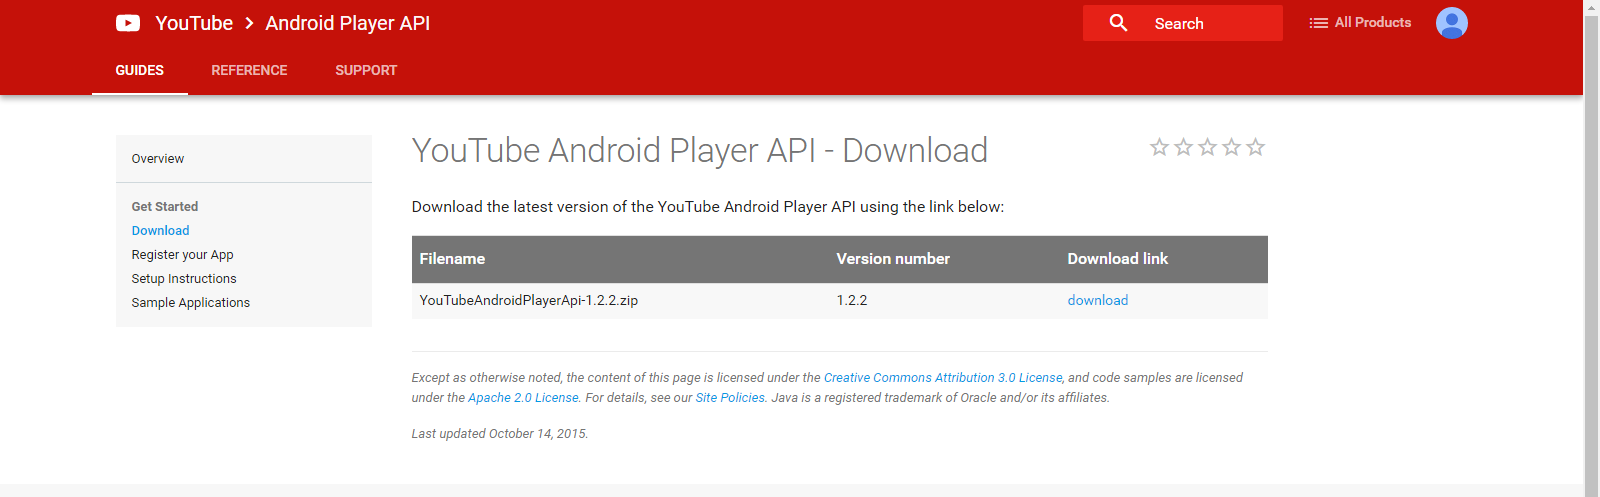
\includegraphics[width=1\textwidth]{gambar/y0}
			\caption{Laman Unduh YouTube Player Android API}
		\end{figure}
		
		\item Kemudian pada Android Studio, ubah tampilan \textit{tree} dari Android menjadi Project dan buat direktori baru bernama \textit{libs} pada direktori \textit{app}
		\begin{figure}[H]
			\centering
			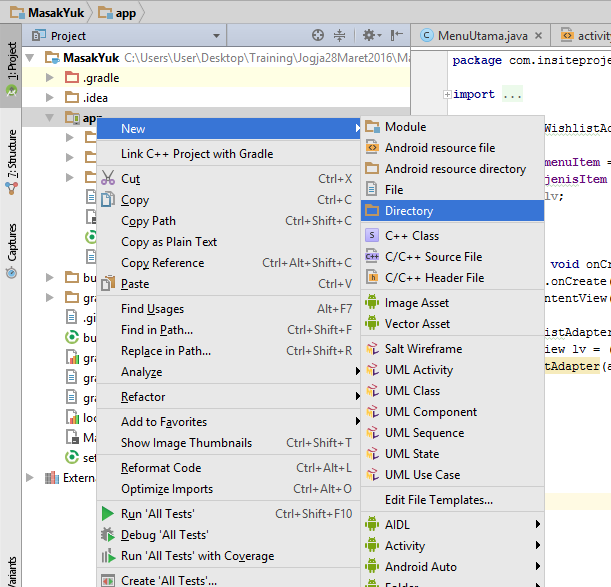
\includegraphics[width=0.8\textwidth]{gambar/y2}
			\caption{Tampilan \textit{tree} Project}
		\end{figure}
		
		\item Ekstrak berkas yang telah diunduh pada langkah pertama dan salin 
		berkas YouTubeAndroidPlayerApi.jar pada direktori \textit{libs}
		\begin{figure}[H]
			\centering
			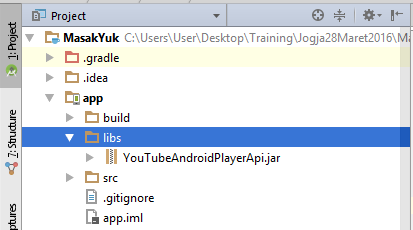
\includegraphics[width=1\textwidth]{gambar/y3}
			\caption{Menyalin Berkas YouTube API}
		\end{figure}	
		
		\item Tambahkan kode compile files('libs/YouTubeAndroidPlayerApi.jar') pada berkas build.gradle yang terdapat di dalam direktori \textit{app}
		\begin{figure}[H]
			\centering
			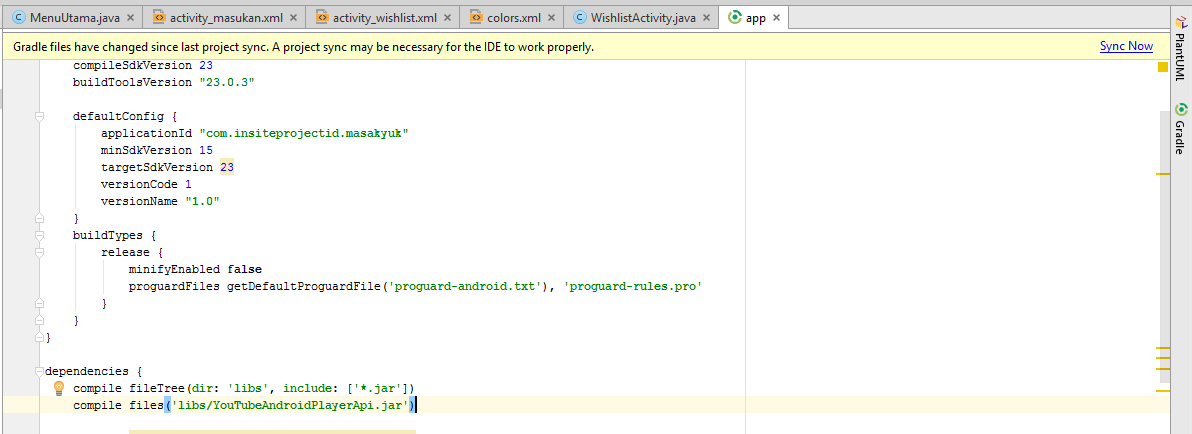
\includegraphics[width=1\textwidth]{gambar/y4}
			\caption{Menambah Baris Kode}
		\end{figure}
	
		\item Akan muncul sebuah pemberitahuan untuk melakukan sinkronisasi pustaka yang ada dengan pustaka YouTube API. Klik \textit{Sync Now} pada pemberitahuan tersebut untuk menginisialisasikan Android dengan YouTube
		\begin{figure}[H]
			\centering
			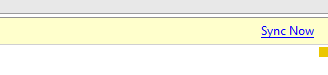
\includegraphics[width=1\textwidth]{gambar/y5}
			\caption{\textit{Sync Now}}
		\end{figure}
		
		\item Buat sebuah Activity dan tambahkan baris kode yang sama dengan kode yang tertera di bawah ini 
		\begin{figure}[H]
			\centering
			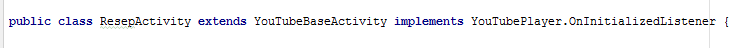
\includegraphics[width=1\textwidth]{gambar/y6}
			\caption{Menambah Baris Kode pada Activity}
		\end{figure}
		
		\item Inisialisasikan YouTubePlayerView pada Activity tersebut
		\begin{figure}[H]
			\centering
			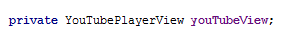
\includegraphics[width=0.6\textwidth]{gambar/y7}
			\caption{Inisialisasi YouTubePlayerView}
		\end{figure}
	
		\item Inisialisasikan juga YouTubePlayerView yang sudah disiapkan pada Activity tersebut ke dalam \textit{method} onCreate.
		\begin{figure}[H]
			\centering
			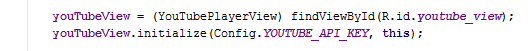
\includegraphics[width=1\textwidth]{gambar/y8}
			\caption{Inisialisasi YouTubePlayerView ke dalam \textit{method} onCreate}
		\end{figure}
		
		\item Pada \textit{layout}, tambahkan baris kode di bawah ini untuk menginisialisasi tampilan YouTube
		\begin{figure}[H]
			\centering
			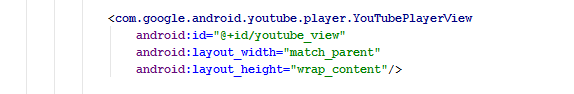
\includegraphics[width=1\textwidth]{gambar/y9}
			\caption{Inisialisasi Tampilan YouTube}
		\end{figure}
		
		\item Implementasikan \textit{method} yang berasal dari API YouTube dengan melakukan klik pada lampu merah yang terdapat pada inisialisasi \textit{class} Activity seperti yang terdapat di bawah ini
		\begin{figure}[H]
			\centering
			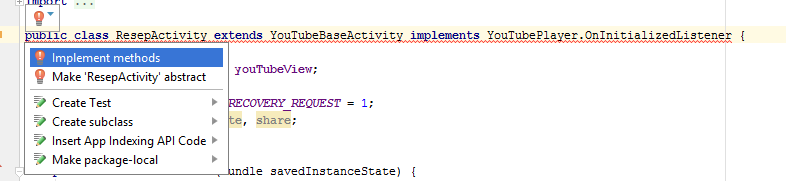
\includegraphics[width=1\textwidth]{gambar/y10-a}
			\caption{Implementasi \textit{Method} YouTube}
		\end{figure}
	
		\item Akan muncul dua \textit{method} penting dalam mengintegrasikan YouTube ke dalam Android, yaitu onInitializationSuccess dan onInitializationFailure seperti di bawah ini 
		\begin{figure}[H]
			\centering
			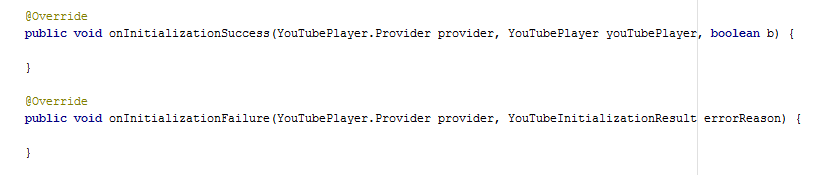
\includegraphics[width=1\textwidth]{gambar/y10}
			\caption{Inisialisasi Tampilan YouTube}
		\end{figure}
		onInitializationSuccess adalah method yang berfungsi untuk menjalankan fitur-fitur YouTube di dalam aplikasi Android apabila inisialisasi sukses. Sedangkan onInitializationFailure adalah metode untuk mengambil alih tindakan yang terjadi apabila YouTube gagal diinisialisasikan.
		
		\item Untuk memutar sebuah video YouTube, API membutuhkan masukan berupa karakter alfanumerik yang terdapat pada akhir dari link YouTube.
		\begin{figure}[H]
			\centering
			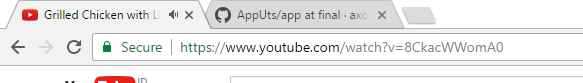
\includegraphics[width=1\textwidth]{gambar/y12}
			\caption{Contoh Karakter Alfanumerik YouTube}
		\end{figure}
		
		Berikut adalah contoh pengaplikasiannya
		\begin{figure}[H]
			\centering
			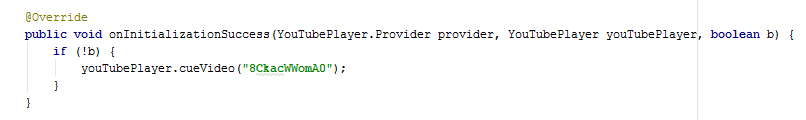
\includegraphics[width=1\textwidth]{gambar/y11}
			\caption{Contoh Pengaplikasian Karakter Alfanumerik YouTube}
		\end{figure}
		
	\end{enumerate}
		
	
	API \emph{client library} berinteraksi dengan sebuah layanan yang terdistribusi sebagai sebuah bagian dari aplikasi YouTube untuk platform Android. \emph{Client library} tersebut meninggalkan sedikit jejak kaki, dengan kata lain tidak akan membebani atau menjadikan ukuran file aplikasi menjadi lebih besar
	


% Baris ini digunakan untuk membantu dalam melakukan sitasi
% Karena diapit dengan comment, maka baris ini akan diabaikan
% oleh compiler LaTeX.
\begin{comment}
\bibliography{daftar-pustaka}
\end{comment}
